\chapter{Self-Supervised Learning}
\label{ssl}

Il \textit{self-supervised learning} (SSL) è una delle strade attualmente più promettenti nell'avanzare la ricerca in ambito di machine learning. Al contrario dell'apprendimento supervisionato, che è spesso fortemente limitato dalla necessità di creare appositi datasets etichettati, la caratteristica principale della SSL è la capacità di \textbf{apprendere} da grandi quantità di \textbf{dati non etichettati}.
Metodi di SSL in computer vision sono stati in grado di pareggiare, e in alcuni casi anche superare modelli allenati tradizionalmente.

Nel corso di questo capitolo si esporranno le principali tecniche e architetture che hanno portato alla nascita di DINOv2, il modello utilizzato nella fase di sperimentazione (Capitolo \ref{risultati}). Tutti i modelli che verranno esposti vengono sviluppati con obiettivo principale quello della classificazione semantica del contenuto delle immagini, utilizzato come task volto alla creazione di features utilizzabili in altri problemi più specifici.

Esiste una risorsa che raccoglie l'evoluzione e gli aspetti più importanti della self-supervision: "\textit{\citefield{cookbook}{title}}" \cite{cookbook} di MetaAI. 

Il \textbf{capitolo non è essenziale ai fini della comprensione della fase sperimentale che segue}, se si considera DINOv2 come un semplice feature extractor. Nonostante ciò, è stato incluso perchè contestualizza la nascita del modello e ne spiega il funzionamento interno, oltre che presentare una panoramica dello studio che è stato condotto durante il periodo di stage.

\section{Cos'è il self-supervised learning}
La self-supervision consiste nella definizione di un \textit{pretext task}, basato su input \textbf{non etichettati}, il cui scopo è la produzione di \textbf{rappresentazioni} degli stessi che siano \textbf{descrittive e intelligibili}. Un pretext task è un obiettivo di pre-training, costruito in base al problema, che viene stabilito per guidare il modello nell'apprendimento di tali rappresentazioni. In ambito di Natural Language Processing, ad esempio, un obiettivo comune è quello di mascherare una parola nel testo e predirre il contesto che la circonda. Questo incoraggia il modello a catturare relazioni fra parole nel testo senza avere bisogno di alcuna label.

Lo scopo ultimo di questi approcci è produrre delle features \textit{general purpose}, utili in una vasta gamma di task. L'ideale è quello di giungere allo sviluppo di \textit{Foundation Models} (FMs): piuttosto che creare da zero delle AI per ciascun task che si desidera risolvere, si vorrebbero introdurre dei modelli allenati su un grande range di dati generali e non etichettati che siano capaci di risolvere compiti disparati con un alto livello di accuratezza. GPT-4 può essere considerato un Foundation Model.

Tutti i modelli che si discuteranno in questo capitolo sono in realtà delle \textbf{tecniche di allenamento} di diverse tipologie di \textit{encoders} (ResNet, Transformer, Vision Transformer). Nel momento in cui la fase di training self-supervised termina, \textbf{si mantiene solamente l'encoder} da utilizzare come \textit{feature extractor} per altri task più specifici, come quello della classificazione della composizione delle immagini.

\subsection{Pro e contro}
Alcuni dei vantaggi della self-supervision rispetto ad approcci supervisionati sono:
\begin{itemize}
    \item Apprendimento di rappresentazioni generiche, utili per una ampia gamma di problemi.
    \item Utilizzo di dati non etichettati:
    \begin{itemize}
        \item La \textbf{disponibilità} di \textbf{dataset etichettati} è \textbf{scarsa} in numero a causa dei tempi di produzione richiesti e costi coinvolti.
        \item L'introduzione di etichette in un dataset \textbf{richiede} la presenza di \textbf{figure professionali} esperte nel settore, che possano correttamente categorizzare i dati coinvolti. Se pensiamo alla creazione di datasets in ambito medico, è inevitabile l'intervento di uno specialista nel definire correttamente le classi di interesse e come assegnarle ai dati. Questo rende datasets etichettati ancora più costosi da produrre.
        \item La quantità di dati esistenti e direttamente accessibili online supera di gran lunga il numero di etichette per gli stessi. Di conseguenza, non avere bisogno di labels permette di \textbf{scalare} notevolmente i propri approcci e allenare su decine, se non centinaia, di milioni di immagini. 
    \end{itemize}
    \item Imparare in autonomia rende i modelli più robusti ad \textit{adversarial examples}, esempi progettati appositamente per ingannare i modelli, e al rumore spesso presente all'interno dei datasets, dovuto in parte anche ad etichettamenti errati o ambigui.
\end{itemize}

Alcuni dei suoi svantaggi:
\begin{itemize}
    \item Il consumo di risorse di tempo ed energia è elevato per l'allenamento di modelli che usano SSL.
    \item Sono richiesti enormi quantità di dati per poter raggiungere valori di accuracy paragonabili alle controparti supervisionate.
    \item Quello della self-supervision è un campo che si basa molto sull'\textbf{evidenza empirica}, essendo ancora in piena fase di sviluppo e ricerca. Spesso vengono presentati risultati in cui si può solo ipotizzare la ragione del successo o insuccesso di un modello, senza conferme provenienti da uno studio teorico.
\end{itemize}

\section{Augmentations}
\label{augmentations}
Gli approcci di SSL si basano in maniera importante sul concetto di \textit{augmentation}. Data una immagine \(X\), con il termine augmentation si indica una versione di \(X\) a cui sono state \textbf{applicate delle trasformazioni}, fra le quali (Figura \ref{fig:augmentations}):
\begin{itemize}
    \item Cropping
    \item Resizing
    \item Rotazione
    \item Flipping
    \item Introduzione di rumore
    \item Introduzione di \textit{blur gaussiano}
    \item Estrazione dell'immagine degli edge tramite filtro di \textit{Sobel}
    \item Diversi tipi di distorsione dei suoi colore
    \begin{itemize}
        \item Trasformare l'immagine da RGB a scala di grigi
        \item Modifiche nella brightness, contrasto, saturazione, tinta
        \item Solarizzazione: inversione del colore di tutti i pixels che hanno un valore sopra una determinata soglia.
    \end{itemize}
\end{itemize}
Quando successivamente si farà riferimento al termine \textit{view} (o vista) di \(X\) si intenderà una augmentation di \(X\).

\vspace{5mm}
\begin{figure}[hb]
    \centering
    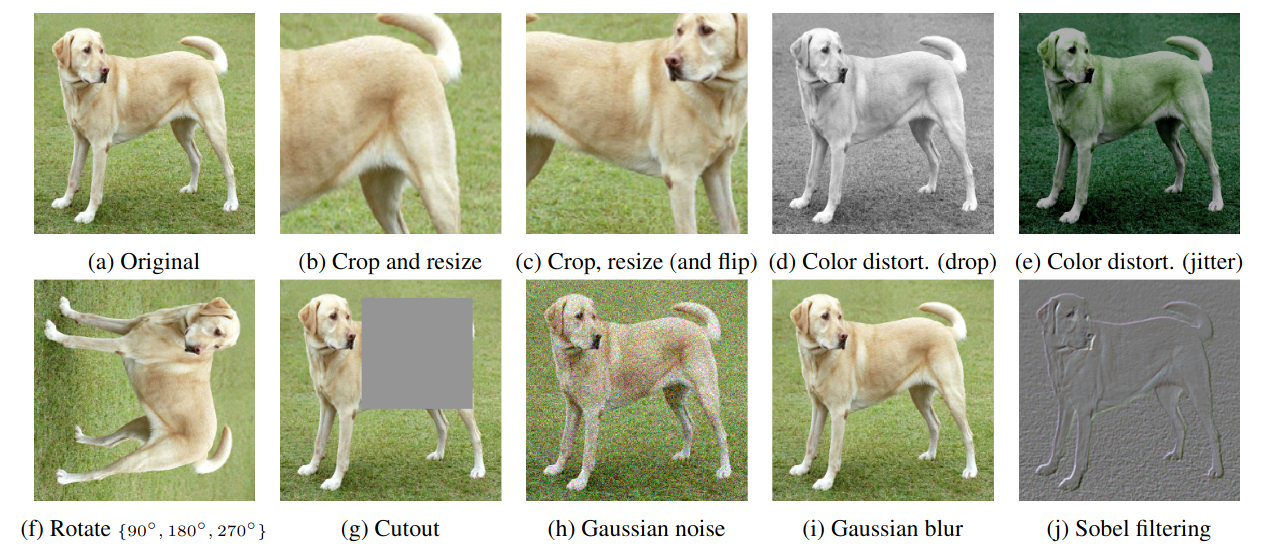
\includegraphics[width=\textwidth]{Immagini/ssl/augmentations.png}
    \caption{Un esempio di alcune delle augmentations più utilizzate in ambito di SSL.}
    \label{fig:augmentations}
\end{figure}

\section{Contrastive Learning}
Il \textit{contrastive learning} è una delle tecniche che stanno alla base della self-supervision.

I metodi supervisionati per i task di classificazione si basano sul confronto fra la classe predetta dal modello e quella reale assegnata al dato, che viene tradotto poi in una funzione di loss che permette al modello di imparare. Nel caso della self-supervision, questo confronto non può avvenire, non esistendo una ground truth. Si devono trovare altri modi per costringere il modello ad apprendere.

Per fare ciò, il contrastive learning introduce il concetto di coppie positive e negative. Data una immagine \(X\):
\begin{itemize}
    \item Coppia \textbf{positiva}: un insieme di due \textit{viste} o augmentations di \(X\), quindi generate a partire dalla stessa immagine.
    \item Coppia \textbf{negativa}: una insieme di due immagini non in relazione fra loro, augmentations non provenienti entrambe da \(X\).
\end{itemize}

L'idea è la seguente. Dato un dataset di immagini, si produce un insieme di augmentations delle stesse. Dopodichè, si formano coppie positive e negative fra le views generate e si allena il modello a differenziare fra le due tipologie, basandosi su determinati criteri di similarità scelti. Gli obiettivi sono:
\begin{itemize}
    \item \textbf{Massimizzare} la \textbf{similitudine fra le rappresentazioni} di immagini provenienti da \textbf{coppie positive}: siccome si tratta di due varianti di una stessa immagine, vogliamo che abbiano vettori di features più vicini possibile.
    \item Massimizzare la distanza fra rappresentazioni in coppie negative, essendo composte da due immagini non correlate fra loro.
\end{itemize}
In questo modo, possiamo stabilire un metro di confronto fra immagini su cui fare \textit{back-propagation} e apprendere, senza avere il bisogno di introdurre labels.

\subsection{SimCLR}
Uno dei modelli più importanti nell'utilizzo della tecnica contrastive è SimCLR (\cite{simclr}), introdotto nel 2020. Di seguito il suo funzionamento.

Durante la fase di training viene scelto casualmente un \textit{minibatch} di \(N\) immagini di esempio dal dataset. Successivamente, per ogni immagine, vengono scelte casualmente due tipologie di augmentation, da un pool di candidati, e vengono applicate. Il risultato sono \(N\) coppie positive e \(2(N-1)\) coppie negative. Le coppie di augmentation \((x_i, x_j)\) vengono passate all'interno della rete.

\begin{figure}[t]
    \centering
    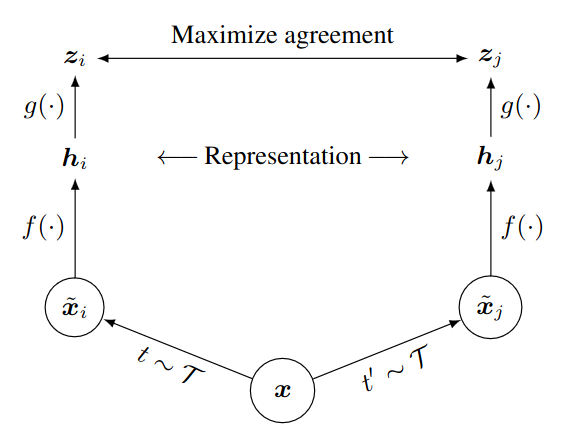
\includegraphics[height=75mm]{Immagini/ssl/arch_simclr.png}
    \caption{Architettura di SimCLR. Questa architettura viene anche detta \textit{siamese}, perchè composta da 2 sotto-reti che condividono architettura e pesi. L'immagine mostra un esempio per coppie positive.}
    \label{fig:arch_simclr}
\end{figure}

\vspace{5mm}

L'architettura si compone di un \textit{encoder f}, cioè una ResNet \cite{resnet} col compito di estrarre una rappresentazione \(h\) dalle immagini, e un projector \(g\), formato da un MLP con 1 layer nascosto e la funzione di attivazione ReLU. Il risultato finale sono due rappresentazioni \((z_i, z_j)\). Il projector viene aggiunto perchè si è verificato sperimentalmente che migliora la performance e la qualità delle features estratte.

A questo punto, per massimizzare l'agreement o la discordanza, la similitudine fra rappresentazioni, viene utilizzata una apposita funzione di \textit{loss contrastiva}.
\begin{equation}
\ell_{i, j} = - \log \frac{exp(sim(z_i, z_j)/\tau)}{\sum^{2N}_{k=1}\mathbb{1}_{k \ne i}exp(sim(z_i, z_k)/\tau)}
\end{equation}
dove 
\begin{equation}
sim(u, v) = \frac{u^Tv}{||u|| \ ||v||}
\end{equation}
è la \textit{cosine similarity} fra i vettori di rappresentazioni, la misura di similitudine scelta per modulare l'agreement, e 
\begin{equation}
    \mathbb{1}_{[k \ne i]} = 
    \begin{cases}
    1 & iff \quad k \ne i \\
    0 & else
    \end{cases}
\end{equation}
La loss risulta essere bassa quando le rappresentazioni delle coppie positive sono simili e quelle delle coppie negative distanti, mentre è alta nella situazione inversa. Questo permette alla rete di imparare correttamente ad aumentare o diminuire le distanze fra le rappresentazioni in base al tipo di coppia, e di conseguenza di imparare delle features che siano robuste, espressive, generalizzanti del contenuto di una immagine, a prescindere dai suoi dettagli più fini di colore, posizione del soggetto, rotazione, e così via.

\subsection{Problemi col contrastive learning}
Il contrastive learning, concepito come SimCLR lo implementa, presenta alcuni problemi, soprattutto quello del trattamento riservato alle coppie negative:
\begin{itemize}
    \item Se le coppie negative sono troppo simili a quelle positive, il rischio è che le rappresentazioni imparate non siano sufficientemente discriminanti, perchè il modello non ha la possibilità di migliorare la propria comprensione di cosa è qualificato come coppia negativa, quale sia la differenza fra le due.
    \item Allo stesso modo, se le coppie negative sono troppo dissimili dai campioni positivi, il pericolo è che si imparino a distinguere solamente le differenze macroscopiche fra due immagini, senza cogliere dettagli piccoli ma rilevanti ai fini della classificazione. 
    \item È richiesto un bilanciamento numerico fra i due tipi di coppie. Come visto in SimCLR, producendo due viste per immagine il risultato è quello di \(N\) coppie positive contro \(2(N-1)\) negative. Questo potrebbe non creare le condizioni adatte affinché si possano imparare features adeguatamente dettagliate, il modello sarebbe in grado di distinguere immagini diverse, ma non di identificare immagini simili. Sarebbe un \textit{overfitting} dei campioni negativi.
\end{itemize}
Per mitigare questi problemi, molti modelli utilizzano strategie quali l'aumentare la dimensione dei batch, utilizzare delle memory banks che memorizzino rappresentazioni di coppie negative da mini-batch precedenti, per diversificare i campioni senza dover necessariamente ripassarli nell'encoder. Altri utilizzano tecniche di \textit{mining} apposite per recuperare esempi negativi migliori.

Un altro aspetto critico è quello della scelta delle augmentations usate. Le performance possono variare drasticamente in base a quali vengono impiegate (Figura \ref{fig:augmentations_simclr}).

\begin{figure}[t]
    \centering
    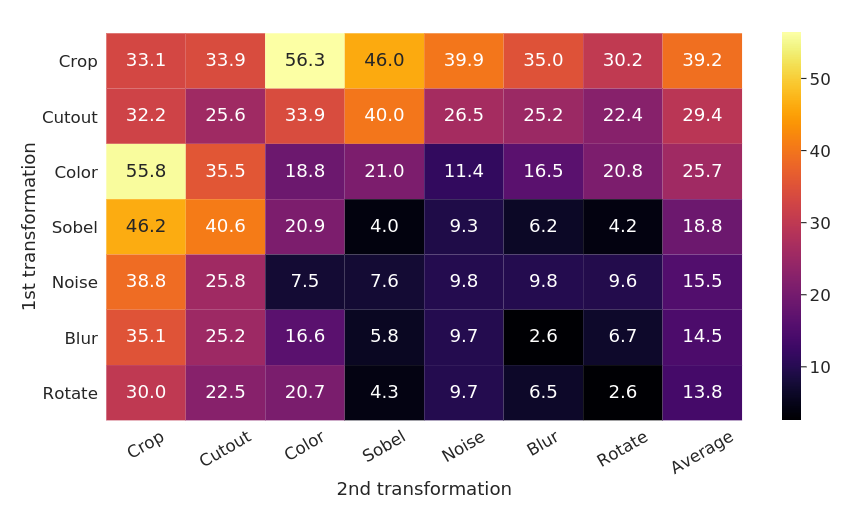
\includegraphics[width=0.7\textwidth]{Immagini/ssl/augmentations_simclr.png}
    \caption{Valori di accuracy di SimCLR al variare delle augmentations scelte per produrre coppie positive e negative. Si nota quanto diverse combinazioni influiscano sulle performance della rete.}
    \label{fig:augmentations_simclr}
\end{figure}

\section{Collasso}
L'idea di base del contrastive learning è efficace, ma come visto, le coppie negative portano con sé diverse criticità a livello gestionale e di performance. Per questo motivo, un corso d'azione che potrebbe risultare naturale seguire è quello di \textbf{utilizzare solamente campioni positivi}. Il problema di questo approccio, però, è che ignorare coppie negative può portare a \textbf{soluzioni banali}: se la rete dovesse imparare la stessa rappresentazione per tutte le immagini che riceve, la loss sarebbe minimizzata, l'obiettivo di massimizzazione della similitudine raggiunto e l'apprendimento interrotto. Questo fenomeno prende il nome di \textit{collasso}, cioè quando una rete \textbf{converge a rappresentazioni non significative}, come un vettore di features dai valori costanti per tutti i samples analizzati.

Secondo il paper "\textit{\citefield{collapse_paper}{title}}" \cite{collapse_paper} esistono due tipologie di collasso, illustrate in Figura \ref{fig:collapse}:
\begin{itemize}
    \item \textbf{Collasso dimensionale}: il vettore di features collassa in uno spazio dimensionale ridotto.
    \item \textbf{Collasso completo}: il vettore di features collassa nell'intorno di un solo punto nello spazio delle rappresentazioni.
\end{itemize}

\begin{figure}[t]
    \centering
    \subcaptionbox{embedding space}{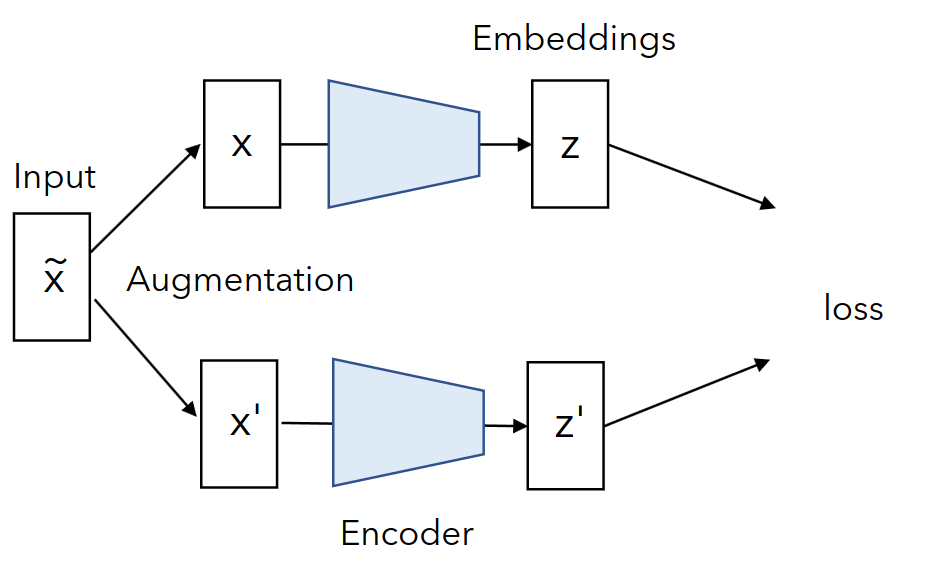
\includegraphics[width=0.43\textwidth]{Immagini/ssl/embedding_space.png}}
    \quad
    \subcaptionbox{dimensionale}{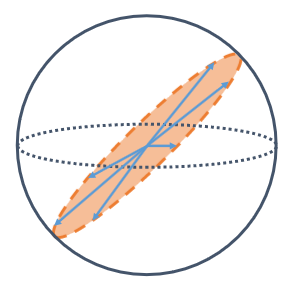
\includegraphics[width=0.24\textwidth]{Immagini/ssl/dimensional_collapse.png}}
    \quad
    \subcaptionbox{completo}{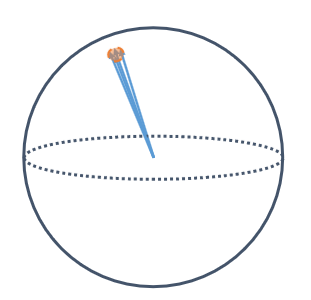
\includegraphics[width=0.26\textwidth]{Immagini/ssl/complete_collapse.png}}
    \caption{Visualizzazione dello spazio delle features nel caso di collasso dimensionale o completo.}
    \label{fig:collapse}
\end{figure}
\vspace{5mm}

Sono nati quindi diversi approcci per contrastare questa problematica, prevalente in tutti i modelli basati su self-supervision, e allo stesso tempo condurre un addestramento che non richieda di coppie negative. Una di queste tecniche è quella di \textit{self-distillation}, su cui si basano tutte le architetture di cui si discuterà, compreso DINOv2.

\section{Self-Distillation}
Il concetto di self-distillation deriva a sua volta da un altro concetto, quello di \textit{knowledge distillation}. 

La distillation (Figura \ref{fig:distillation}) è una tecnica utilizzata in deep learning che permette di \textbf{trasferire la conoscenza appresa} da un modello pre-allenato di grandi dimensioni, detto \textit{Teacher}, ad un modello di dimensioni ridotte e ancora da allenare, detto \textit{Student}. In pratica, lo \textbf{student} deve imparare a \textbf{riprodurre le distribuzioni di probabilità} prodotte \textbf{del teacher} relativamente alle classi predette, a fronte dello stesso dato in input (immagini nel nostro caso). L'obiettivo di questa tecnica è ottenere un modello più piccolo, ma dalle performance comparabili a quelle del Teacher, con minori requisiti computazionali e di memoria. Questo aspetto è particolarmente utile per importare reti su dispositivi con risorse limitate, come smartphones o dispositivi IoT.

\begin{figure}[t]
    \centering
    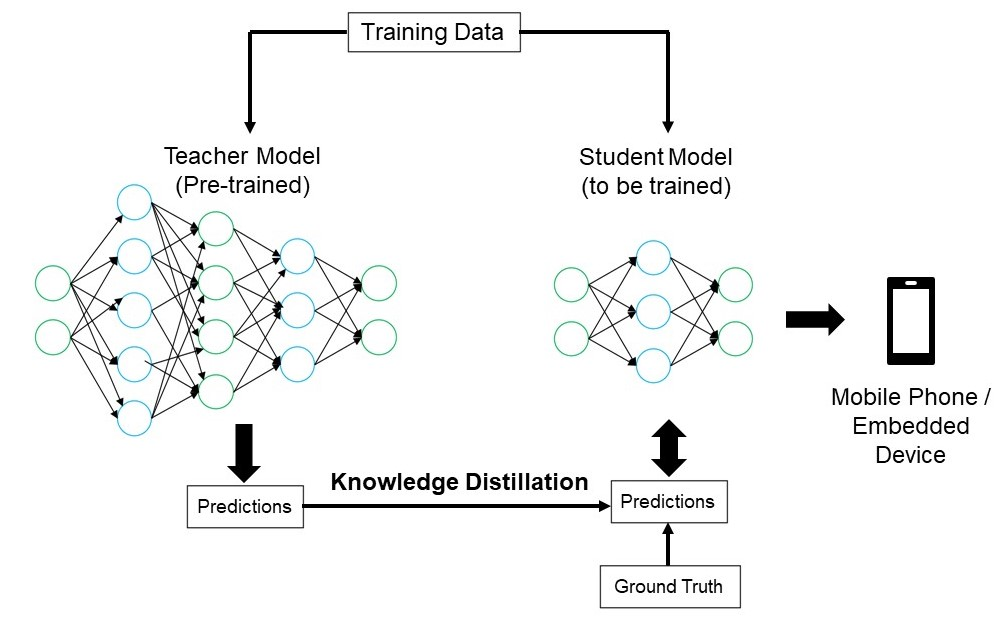
\includegraphics[width=0.75\textwidth]{Immagini/ssl/distillation.jpg}
    \caption{Visualizzazione del workflow utilizzato nella knowledge distillation.}
    \label{fig:distillation}
\end{figure}

In ambito di self-supervision, non è tanto l'aspetto relativo alle risorse a interessarci, quanto piuttosto la \textbf{struttura della rete} per il trasferimento di conoscenza. L'idea è quella di introdurre \textbf{una} prima \textbf{rete} neurale, inizializzata casualmente, che \textbf{produca una rappresentazione target} per ciascuna view, e \textbf{una seconda} rete \textbf{allenata a replicarli}, data un'altra view della stessa immagine. Questi due ruoli possono essere ricoperti da un Teacher e uno Student, come nella distillation. Una volta terminato l'allenamento della rete, il Teacher viene scartato, e le features prodotte dallo Student saranno quelle definitive.

Si dimostra empiricamente che questo approccio funziona realmente nell'evitare il collasso, ma con un grande compromesso: le rappresentazioni risultanti, prodotte dalla rete Student, sono inadeguate e di bassa qualità. È un risultato prevedibile, avendo allenato una rete ad approssimare il Teacher, che è stato inizializzato casualmente e che non ha modo a sua volta di apprendere. Nonostante ciò, si è verificato sperimentalmente che una rete Student che replica delle rappresentazioni casuali performa meglio, in termini di accuracy nella classificazione, di una rete inizializzata casualmente (18.8\% contro 1.4\% su ImageNet, rispettivamente, sul modello BYOL, di cui si parlerà a breve). Questo fenomeno è evidenza del fatto che qualcosa di significativo viene effettivamente appreso, pure essendo il Teacher una rete casuale. 

Per risolvere il problema del collasso e permettere allo stesso tempo allo student di imparare features di qualità, si introduce la \textit{self-distillation}. Si \textbf{ripete} il processo di \textbf{distillation} più volte, fino alla convergenza della rete, imponendo come \textbf{nuovi targets} da replicare le \textbf{rappresentazioni prodotte dallo student all'iterazione precedente}. L'aspettativa è quella di costruire mano a mano delle features che siano sempre più accurate, evitando contemporaneamente il collasso. L'aggiornamento del teacher viene fatto tramite una \textit{Exponential Moving Average} (EMA) dei pesi della rete studente. In questa configurazione, lo student viene anche detta rete \textit{online}. Notare sempre che non è una soluzione definitiva al collasso, ma una evidenza empirica che i ricercatori hanno osservato nel costruire i loro modelli, fra cui BYOL.

\subsection{BYOL}
\textit{Bootstrap your own latent} \cite{byol} è il modello che introduce l'approccio di self-distillation, che viene declinato nell'architettura in Figura \ref{fig:arch_byol}.

La rete si compone di un encoder \(f\), di un projector \(g\), formato da un MLP con 1 layer hidden e funzione di attivazione ReLU, e predictor \(q\), con la stessa struttura di \(g\), ma presente solo nello student, avendo il compito di predirre le rappresentazioni del teacher.

L'aggiornamento dei pesi del teacher tramite EMA dei pesi dello studente viene anche detto \textit{Momentum Encoder}, e viene fatto come segue:
\begin{equation}
    \xi \gets \tau \xi + (1-\tau)\theta
\end{equation}
dove:
\begin{itemize}
    \item \(\xi\) sono i pesi del teacher
    \item \(\theta\) sono i pesi dello student
    \item \(\tau\) è un \textit{momentum coefficient} compreso in \([0, 1]\), che nel caso di BYOL vale inizialmente 0.996 e sale a 1 durante l'allenamento. Il risultato è che il Teacher viene aggiornato principalmente nelle prime iterazioni, fino ad arrivare al punto in cui i suoi pesi vengono fissati e l'allenamento viene fatto solo sullo Student. Lo \textit{stop gradient} posto in cima al teacher impedisce ai pesi di essere aggiornati tramite back-propagation.
\end{itemize}
\vspace{5mm}
\begin{figure}[!t]
    \centering
    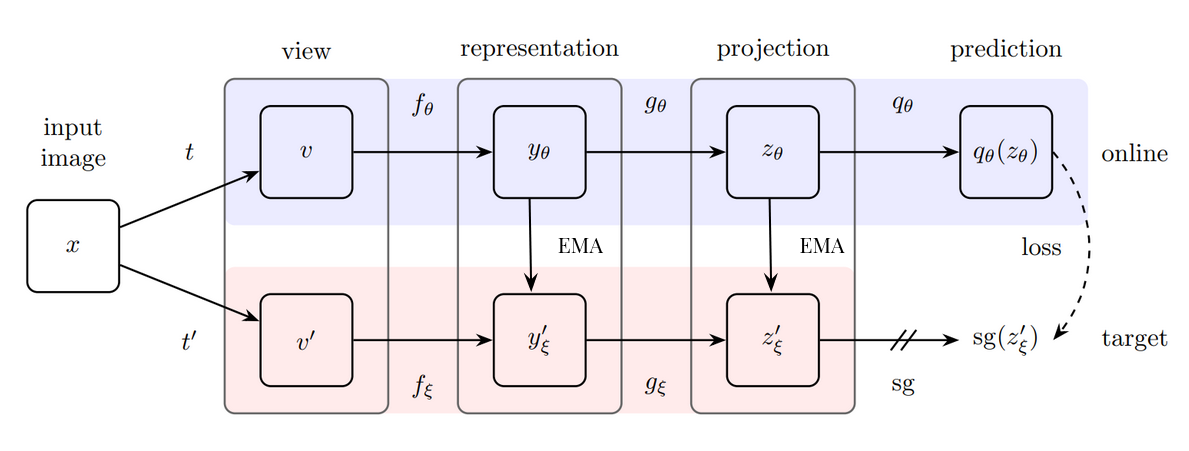
\includegraphics[width=\textwidth]{Immagini/ssl/arch_byol.png}
    \caption{Architettura di BYOL.}
    \label{fig:arch_byol}
\end{figure}
La loss utilizzata è una MSE fra la predizione dello Student e la rappresentazione corrispondente del Teacher.
\begin{equation}
    L_{\theta, \xi} = || \overline{q_{\theta}}(z_\theta) - \overline{z}'_\theta||^2
\end{equation}
dove \(\overline{q_\theta}(z_\theta)\) è il vettore di predizioni dello Student l2-normalizzato e \(\overline{z}'_\theta\) è il vettore proiettato del Teacher l2-normalizzato. Questo è il calcolo per una sola coppia di augmentations, a partire da una sola immagine. Per effettuare la back-propagation si dovranno mediare tutti i risultati di loss ottenuti in un batch.

Inoltre, la loss viene simmetrizzata, come mostrato in Figura \ref{fig:byol_loss}. La loss reale sarà \(L^{BYOL}_{\theta, \xi} = L_{\theta, \xi} + \Tilde{L}_{\theta, \xi}\). Simmetrizzare permette di avere più samples su cui fare addestramento, in maniera efficiente.

Per quanto riguarda il collasso, gli autori osservano che la combinazione di teacher e predictor effettivamente previene la problematica: rimuovere uno dei due risulta realmente nel collasso della rete.

\begin{center}
\begin{figure}[b]
    \centering
    \begin{tikzpicture}
        % Definisci i nodi
        \node[draw, rectangle, rounded corners=5pt, inner sep = 10pt] (x) {\(x\)};
        \node[draw, rectangle, rounded corners=5pt, right=of x, inner sep = 10pt, yshift = 1.0cm, xshift = 0.6cm] (v) {\(v\)};
        \node[draw, rectangle, rounded corners=5pt, right=of x, inner sep = 10pt, yshift = -1.0cm, xshift = 0.6cm] (v') {\(v'\)};
        \node[draw, rectangle, rounded corners=5pt, right=of v, inner sep = 10pt, xshift = 1cm] (student) {Student};
        \node[draw, rectangle, rounded corners=5pt, right=of v', inner sep = 10pt, xshift = 1cm] (teacher) {Teacher};
        \node[draw, rectangle, rounded corners=5pt, right=of student, inner sep = 10pt, xshift = 1cm] (l1) {\(L_{\theta, \xi}\)};
        \node[draw, rectangle, rounded corners=5pt, right=of teacher, inner sep = 10pt, xshift = 1cm] (l2) {\(\Tilde{L}_{\theta, \xi}\)};
    
        % Disegna le frecce
        \draw[->] (x) -- (v);
        \draw[->] (x) -- (v');
        
        \draw[->, color=red, line width =  0.6mm] (v) -- (student);
        \draw[->, color=red, line width =  0.6mm] (v') -- (teacher);
        \draw[->, color=red, line width =  0.6mm] (student) -- (l1);
        \draw[->, color=red, line width =  0.6mm] (teacher) -- (l1);
    
        \draw[->, color=blue, line width =  0.6mm] (v') -- (student);
        \draw[->, color=blue, line width =  0.6mm] (v) -- (teacher);
        \draw[->, color=blue, line width =  0.6mm] (student) -- (l2);
        \draw[->, color=blue, line width =  0.6mm] (teacher) -- (l2);
  
    \end{tikzpicture}
    \caption{Workflow per il calcolo della loss simmetrizzata.}
    \label{fig:byol_loss}
\end{figure}
\end{center}
Un confronto con SimCLR si trova in Figura \ref{tab:res-byol}. Inoltre, gli autori verificano che BYOL è molto meno influenzato dalla dimensione dei batch e dalla scelta delle augmentations, raggiungendo l'obiettivo prefissato.

\begin{table}[t]
    \centering
    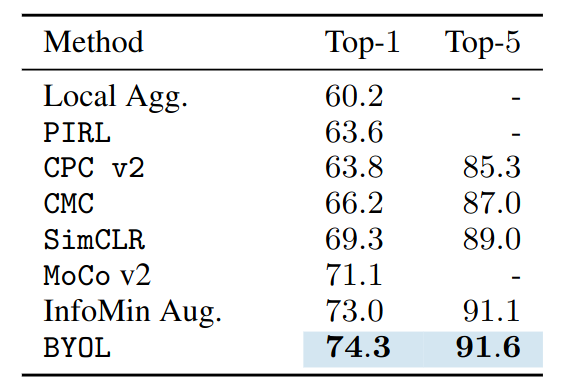
\includegraphics[height=50mm]{Immagini/ssl/res_byol.png}
    \caption{Confronto top-1 e top-5 accuracies in linear evalutation su ImageNet usando una ResNet-50 come encoder fra BYOL e altri metodi di SSL. Si nota come BYOL migliori in maniera rilevante le prestazioni di SimCLR e altri modelli concorrenti.}
    \label{tab:res-byol}
\end{table}


\section{DINO}
DINO (\textit{self-\textbf{di}stillation with \textbf{no} labels}) \cite{dino} è stato il tentativo da parte di Meta di \textbf{conciliare} l'evoluzione della \textbf{self-supervision}, in particolare della self-distillation, con il recente avvento dei Transformers \cite{transformer} in ambito di NLP, \textbf{e} conseguentemente dei \textbf{Vision Transformers} (ViT). Per maggiori dettagli su queste due architetture, leggere Appendice \ref{appendice_transformers}.

L'osservazione che fanno i creatori di DINO è che i ViT sono competitivi con le CNN, ma non mostrano chiari benefici che li rendano una scelta migliore, considerato che:
\begin{itemize}
    \item Richiedono maggiori quantità di dati
    \item Sono più costosi in termini di risorse computazionali
    \item Le features che producono non hanno proprietà particolari. Nelle CNN sappiamo che i primi layers della rete estraggono features di basso livello, come potrebbero essere gli edges, e andando sempre più in profondità si costruiscono features progressivamente più complesse. Nei ViT non abbiamo lo stesso tipo di sicurezza nell'interpretare gli output intermedi della rete.
\end{itemize}
L'ipotesi formulata è che il \textbf{colpevole} di questa mancanza di progresso possa essere la \textbf{supervisione}, con cui i ViT sono stati allenati fino a questo punto. La supervisione riduce il ricco contenuto visuale di una immagine a un singolo concetto in un insieme predefinito di categorie, in cui lo classifichiamo. Da qui nasce l'idea di utilizzare la self-distillation, come definito precedentemente, per allenare un vision transformer in maniera self-supervised.

L'intuizione di Meta ha avuto successo, le features prodotte dal ViT \textbf{contengono esplicitamente} informazioni sul layout della scena nell'immagine, e in particolare, la \textbf{segmentazione} dei suoi oggetti (Figura \ref{fig:dino_attention}). Questa informazione è direttamente accessibile tramite i \textbf{blocchi di self-attention} che caratterizzano il funzionamento di un transformer (Sezione \ref{self-attention}). Le features prodotte sono tanto buone da competere con altri modelli nello stato dell'arte con un semplice classificatore kNN.

\vspace{5mm}

\begin{figure}[t]
    \centering
    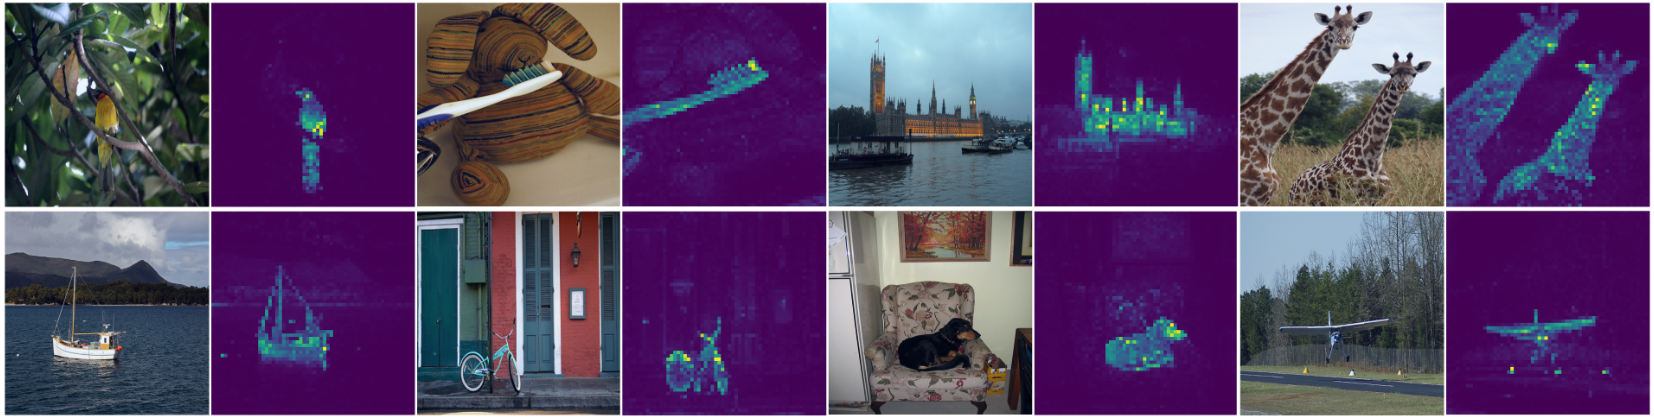
\includegraphics[width=\textwidth]{Immagini/ssl/dino_attention.png}
    \caption{Mappe di self-attention estratte dal token [CLS], sulle teste del blocco di \textit{multi-head attention} dell'ultimo layer.}
    \label{fig:dino_attention}
\end{figure}

\subsection{Dettagli implementativi}
Come nei modelli precedenti, a partire da una immagine \(x\) si producono delle augmentations. Nel caso di DINO si usa la tecnica del \textit{multi-crop}. Oltre alle trasformazioni già viste nella Sezione \ref{augmentations}, si introducono i concetti di:
\begin{itemize}
    \item Vista \textit{locale}: crop dell'immagine di dimensione inferiore al 50\% rispetto a quella originale
    \item Vista \textit{globale}: crop di dimensione \(\geq 50\)\%
\end{itemize}
Il \textbf{Teacher riceve} in input \textbf{solamente viste globali}, mentre lo student entrambi i tipi. Questo è significativo perchè, siccome il teacher conosce solamente immagini che ricoprono più di metà delle controparti originarie e siccome lo \textbf{student} impara direttamente da esso, quest'ultimo viene \textbf{costretto a imparare feature più generali} anche da crop piccoli, evitando di concentrarsi eccessivamente su dettagli fini e irrilevanti ai fini della classificazione.
\vspace{-1.1cm}
\begin{center}
    \begin{figure}[b]
        \centering
        \begin{tikzpicture}
        % Definisci i nodi
        \node[draw, rectangle, rounded corners=5pt, inner sep = 10pt] (image) {Image};
        \node[draw, rectangle, rounded corners=5pt, right=of x, inner sep = 10pt, xshift = 0.6cm] (augmented) {Augmented};
        \node[draw, rectangle, rounded corners=5pt, right=of augmented, inner sep = 10pt, yshift= 1cm, xshift = 0.6cm] (global) {2x Global};
        \node[draw, rectangle, rounded corners=5pt, right=of augmented, inner sep = 10pt,  yshift= -1cm, xshift = 0.6cm] (local) {6x Local};
        \node[draw, rectangle, rounded corners=5pt, right=of global, inner sep = 10pt, xshift = 0.6cm] (teacher) {Teacher};
        \node[draw, rectangle, rounded corners=5pt, right=of local, inner sep = 10pt, , xshift = 0.9cm] (student) {Student};
    
    
        % Disegna le frecce
        \draw[->, line width =  0.6mm] (image) -- (augmented);
        \draw[->, line width =  0.6mm] (augmented) -- (global);
        \draw[->, line width =  0.6mm] (augmented) -- (local);
        \draw[->, line width =  0.6mm] (global) -- (teacher);
        \draw[->, line width =  0.6mm] (global) -- (student);
        \draw[->, line width =  0.6mm] (local) -- (student);
        
    
        \end{tikzpicture}
        \vspace{3mm}
        \caption{Workflow per multi-cropping. A partire da una immagine vengono prodotte 2 viste globali e 6 viste locali. In questo modo aumentano i samples senza ricalcolare altre augmentations.}
        \label{fig:multicrop}
    \end{figure}
\end{center}

L'architettura della rete è esposta in Figura \ref{fig:arch_dino}. Teacher e Student si compongono entrambi di un ViT, con pesi diversi, e un projector. Rimane il momentum encoder, ma al posto del predictor, per evitare il collasso, si introducono due novità all'output del Teacher, complementari fra loro:
\begin{itemize}
    \item \textbf{Centering}: evita che una sola dimensione nello spazio delle features possa dominare (collasso dimensionale), ma ha come effetto collaterale l'uniformare le rappresentazioni (collasso completo). Viene realizzato aggiungendo un bias \(c\) a tutte le predizioni del teacher:
    \begin{equation}
    g_t \gets g_t(x) + c
    \end{equation}
    dove \(c\) viene aggiornato come una exponential moving average dei pesi del teacher
    \begin{equation}
    c \gets mc + (1-m)\frac{1}{B}\sum^B_{i=1}g_{\theta_t}(x_i)
    \end{equation}
    con \(m\) parametro che decide il rate di aggiornamento, \(B\) è la dimensione del batch, \(x_i\) immagine nel batch.
    \item \textbf{Sharpening}: al contrario del centering, evita una distribuzione costante, ma può causare il dominio di una dimensione. Viene fatto utilizzando un valore di \textit{temperatura} basso \(0.04 < \tau < 0.07\) nel calcolo del softmax:
    \begin{equation}
    \scalebox{1.2}{$P_i = \frac{e^{\frac{y_i}{\tau}}}{\sum^n_{k=1}e^{\frac{y_k}{\tau}}}$}
    \end{equation}
    dove \(y_i\) indica l'attivazione della classe i-esima. Un \(\tau\) basso fa in modo che la distribuzione di probabilità risultante sia più decisa nelle sue predizioni, meno uniforme.
\end{itemize}

\begin{figure}[t]
    \centering
    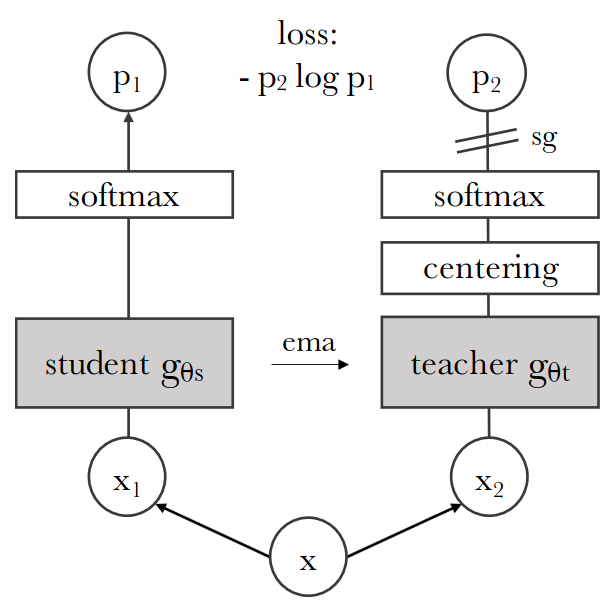
\includegraphics[height=70mm]{Immagini/ssl/arch_dino.png}
    \caption{Architettura di DINO. Rete teacher e student hanno stessa architettura, ma parametri diversi, come BYOL.}
    \label{fig:arch_dino}
\end{figure}

Infine, la loss utilizzata è una \textit{cross-entropy loss}, con la quale lo Student cerca di riprodurre la distribuzione di probabilità generata dal Teacher:
\begin{equation}
\underset{\theta_s}{\min} \sum_{x \in \{x_1^g, x_2^g\}}\sum_{x' \in V, x' \ne x} H(P_t(x), P_s(x'))
\end{equation}
con \(H(a, b) = -a \log b\), \(x^g\) vista globale, \(V\) insieme di tutte le viste, \(a\) distribuzione di probabilità da replicare (Teacher), \(b\) distribuzione di probabilità predetta (Student).

\begin{table}[t]
    \centering
    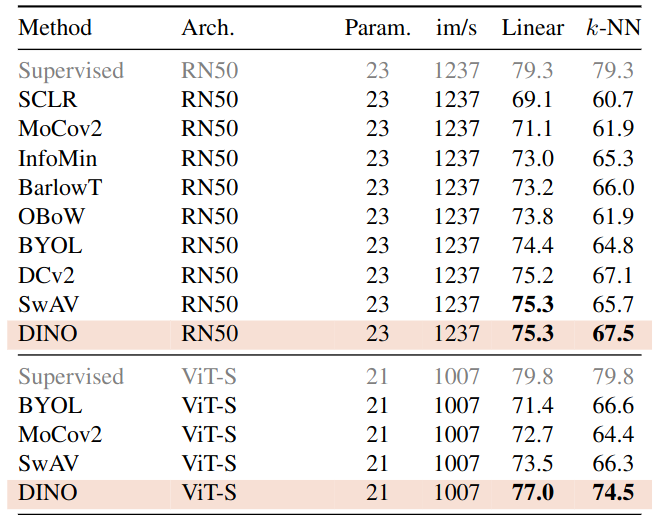
\includegraphics[height=70mm]{Immagini/ssl/res_dino.png}
    \caption{Confronto top-1 accuracy per linear e kNN sul validation set di ImageNet fra DINO e diversi altri metodi di self-supervision. In grigio i risultati supervisionati, in arancione quelli di DINO.}
    \label{fig:res_dino}
\end{table}

\section{Migliorare DINO}
DINO migliora lo stato dell'arte in ambito di self-supervision, ma le sue \textbf{performance} risultano ancora \textbf{inferiori rispetto a metodi supervisionati} tradizionali (vedi Figura \ref{fig:res_dino}). Uno dei modelli emersi nel tentativo di evolvere l'approccio adottato da DINO è stato iBOT \cite{ibot}.

\subsection{BERT}
L'idea dei ricercatori dietro iBOT è stata quella di prendere ispirazione dal natural language processing, in particolare da BERT \cite{bert}, un'evoluzione dei transformer nata nel 2018. La particolarità di BERT sta nel suo paradigma di pre-training, che prende il nome di \textit{masked language modeling} (MLM). Questo consiste nel \textbf{mascherare casualmente alcuni dei tokens in input al transformer}, con obiettivo quello di predirre l'ID nel vocabolario della parole che sono state mascherate, basandosi solo sul contesto fornito dalla frase. Questo approccio permette di risolvere una problematica dei transformers, ovvero che le parole vengono processate in una sola direzione, da sinistra verso destra, limitando la capacità espressiva delle features. Nei transformer tradizionali, la parte di frase analizzata finora viene utilizzata nella predizione del prossimo token, e se fosse consentita una analisi bidirezionale della frase, il modello avrebbe visibilità delle parole che deve predirre, portando a soluzioni banali. MLM risolve il problema sostituendo una parte delle parole nella frase con il token [MASK] e utilizzando una testa di classificazione per ciascuno di essi per allenare la rete a ricostruire la parola originaria.

\subsection{iBOT}
\begin{figure}[!t]
    \centering
    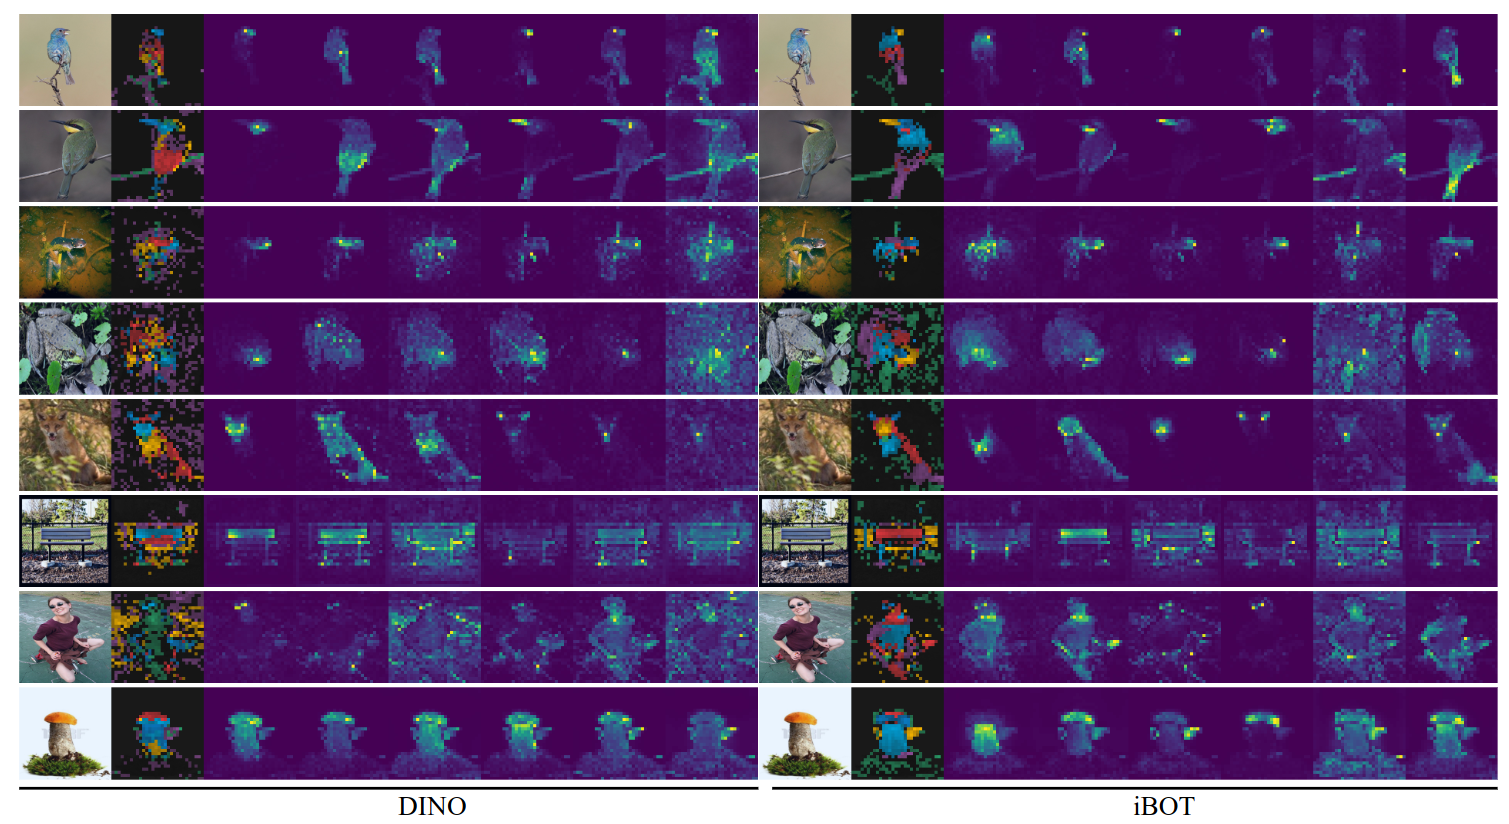
\includegraphics[width=\textwidth]{Immagini/ssl/ibot_vs_dino.png}
    \caption{Confronto fra le teste di self-attention per il token [CLS] in iBOT e DINO. Si nota come le segmentazioni prodotte da iBOT siano più precise e meno rumorose, e come ciascuna testa rilevi un singolo particolare dettaglio dell'immagine relativa, in maniera più granulare rispetto DINO.}
    \label{fig:ibotvsdino}
\end{figure}
iBOT (\textit{\textbf{i}mage \textbf{B}ERT pre-training with \textbf{O}nline \textbf{T}okenizer}) si ispira a DINO nella sua architettura e a BERT nel stabilire il suo pretext task, che prende il nome di \textit{masked image modeling} (MIM). Data una immagine \(x=\{x_i\}^N_{i=1}\), dove \(N\) è il numero di patches in cui è suddivisa (siamo sembre in ambito di ViT), MIM crea una \textbf{maschera binaria casuale} \(m \ \in \{0, 1\}^N\). Se il patch \(x_i\) ha corrispondente valore in \(m_i\) pari a 1, allora quel patch viene sostituito col token [MASK]. L'\textbf{obiettivo} diventa quello di \textbf{recuperare le rappresentazioni corrette dei token mascherati}, a partire dall'immagine corrotta. La predizione, quindi, non viene fatta a livello di pixels dell'immagine, approccio che usano i \textit{Masked Auto Encoders} (MAE), ma nello spazio delle features. Apprendere rappresentazioni per i token mascherati usando il contesto che li circonda \textbf{conduce a delle features} ancora \textbf{più ricche di significato} rispetto a quelle di DINO (Figura \ref{fig:ibotvsdino}).


L'architettura della rete (Figura \ref{fig:arch_ibot}) rimane simile a quella di DINO, mantenendo la struttura di self-distillation con Student e Teacher e momentum encoder. Il teacher viene anche detto \textit{online tokenizer} e il motivo è che \textbf{solo lo student riceve in input i patches mascherati}. Il \textbf{ruolo del teacher} è quello di \textbf{produrre le rappresentazioni per il token [MASK] che lo student dovrà replicare}. Si ricostruiscono i token mascherati con la supervisione del teacher.

\begin{figure}[!t]
    \centering
    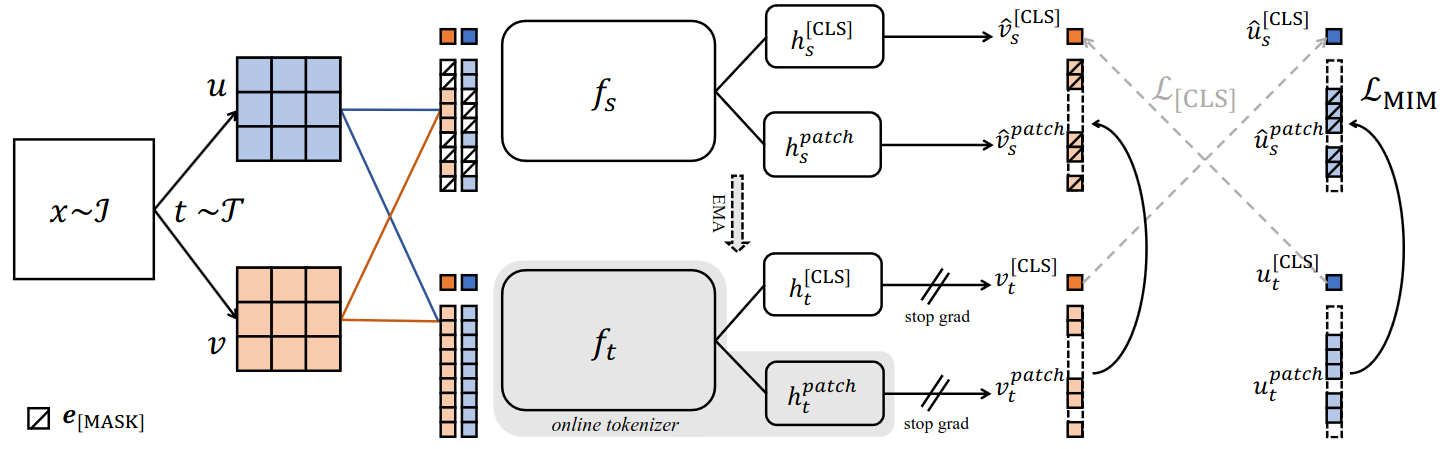
\includegraphics[width=\textwidth]{Immagini/ssl/arch_ibot.png}
    \caption{Architettura di iBOT. \(h_s^{[CLS]}\) e \(h_s^{patch}\) condividono i pesi, così come \(h_t^{[CLS]}\) e \(h_t^{patch}\). L'input dello Student viene mascherato solo per l'obiettivo MIM, non per la costruzione di CLS.}
    \label{fig:arch_ibot}
\end{figure}

Date due viste \(u\) e \(v\) della stessa immagine \(x\), ogni vista passa attraverso i ViT \(f_s\) e \(f_t\). Seguono delle teste di proiezione \(h\) formate da un MLP a 3 layer. Gli autori provano empiricamente che condividere i pesi delle teste \(h^{[CLS]}\) e \(h^{patch}\) conduce a risultati migliori, in quanto la semantica ottenuta nella distillation su [CLS] può dare informazione in più nel completare l'obiettivo MIM.

La loss si compone della somma di due cross-entropy: 
\begin{equation}
\mathcal{L} = \mathcal{L}_{[CLS]} + \mathcal{L}_{MIM}
\end{equation}
dove \(\mathcal{L}_{[CLS]}\) è la distillazione sul token CLS del ViT ed è simmetrizzata (come BYOL, Figura \ref{fig:byol_loss}) 
\begin{equation}
\mathcal{L}_{CLS} = -P_{\theta'}^{[CLS]}(v)^T \log P_{\theta}^{[CLS]}(u)
\label{eq:loss_cls}
\end{equation} 

con \(\theta'\) i pesi del teacher e \(\theta\) quelli dello student, e \(\mathcal{L}_{MIM}\) è la somma delle loss calcolate fra i patch [MASK] e le rappresentazioni dei rispettivi token prodotte dal teacher:
\begin{equation}
    \mathcal{L}_{MIM} = -\sum_{i=1}^N m_i \cdot P_{\theta'}^{patch}(u_i)^T \log P_{\theta}^{patch}(\hat{u}_i)
    \label{eq:loss_mim}
    \end{equation}

iBOT migliora DINO (Figura \ref{fig:res_ibot}) in termini di accuracy, ma è anche maggiormente scalabile, presentando un guadagno in performance maggiore all'aumentare del numero dei parametri.
\vspace{1cm}
\begin{figure}[h]
    \centering
    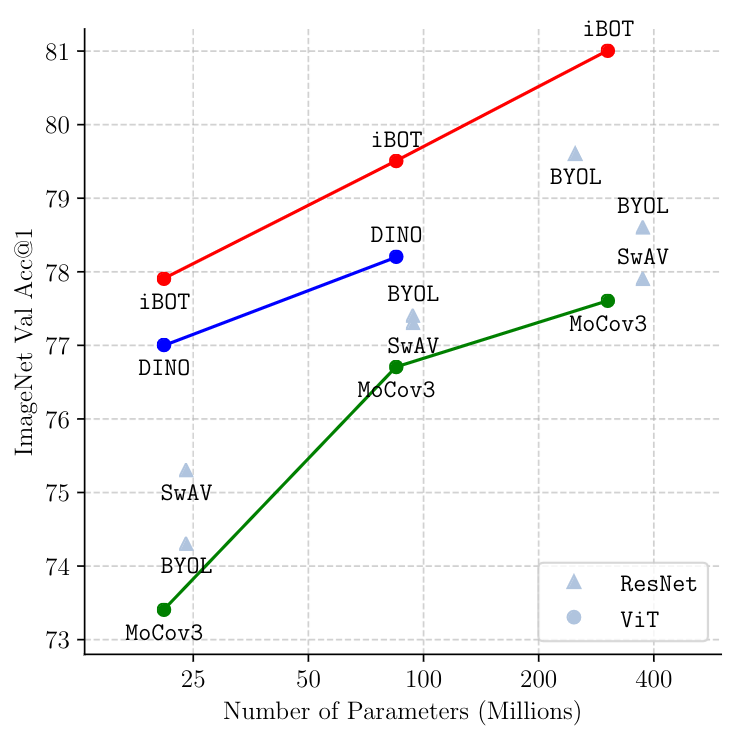
\includegraphics[height=80mm]{Immagini/ssl/res_ibot.png}
    \caption{Confronto fra iBOT e altri modelli self-supervised. iBOT supera le prestazioni della concorrenza.}
    \label{fig:res_ibot}
\end{figure}

\clearpage
\section{DINOv2}
\label{dinov2}
DINOv2 \cite{dinov2} viene pubblicato nell'aprile 2023 come una versione nuova e migliorata del suo predecessore del 2021, costruendo sulla base lasciata da iBOT. Mira ad \textbf{accelerare e stabilizzare il training su grande scala} di DINO, introducendo diverse \textbf{migliorie e ottimizzazioni nei suoi componenti più tecnici}, come il calcolo della attention o dello \textit{stochastic gradient descent}, che non si andranno ad approfondire in questo elaborato.

\subsection{LVD-142M}
\label{LVD}
Un aspetto importante dell'innovazione portata da DINOv2 è l'introduzione di un \textbf{dataset curato e personalizzato} da utilizzare in fase di pre-training del modello. L'importanza di ciò è data dal fatto che la maggior parte degli avanzamenti in ambito di SSL sono stati fatti nel contesto di datasets di dimensioni ridotte, frequentemente su ImageNet-1k, che contiene 1.2 milioni di immagini nel suo split di training, circa 1300 per ciascuna delle sue mille classi. I tentativi di scalare questi approcci con \textbf{datasets non curati} di dimensioni maggiori ha portato inevitabilmente ad un \textbf{calo di qualità nelle features} a causa della \textbf{assenza di controllo sulla diversità} delle immagini in questi datasets e della loro \textbf{qualità}. Per questo motivo, viene costruito il dataset \textit{LVD-142M}, che come dice il nome, si compone di un totale di 142 milioni di immagini, provenienti da sorgenti curate e non. La pipeline utilizzata per costruirlo è meglio spiegata nel paper \cite{dinov2}, di seguito una overview:
\begin{figure}[b]
    \centering
    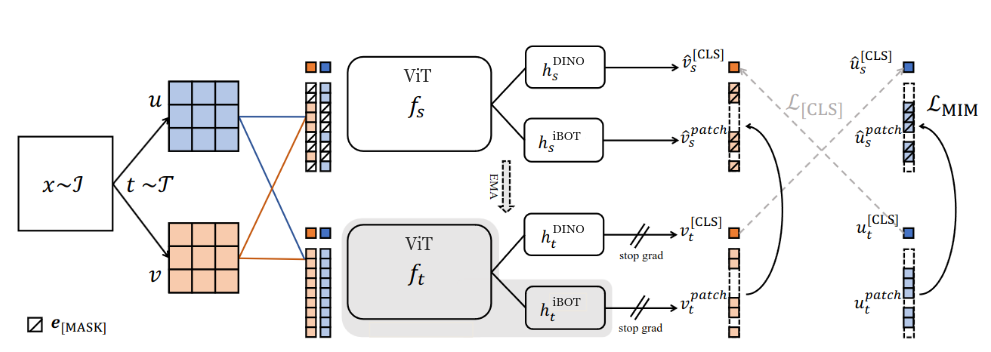
\includegraphics[width=\textwidth]{Immagini/ssl/arch_dinov2.png}
    \caption{Architettura di DINOv2. È la stessa di iBOT (Figura \ref{fig:arch_ibot}, con la differenza che i pesi delle teste sono separati questa volta.}
    \label{fig:arch_dinov2}
\end{figure}\textbf{}
\begin{itemize}
    \item \textbf{Sorgenti}: si raccolgono più di 1.2 miliardi di immagini, prese da sorgenti curate (diverse varianti di ImageNet, Google Landmarks, Food-101, Caltech 101, e altri) e sorgenti non curate, ottenute tramite web scraping.
    \item \textbf{Deduplication}: si utilizza la pipeline di \textit{copy detection} di Pizzi et al. \cite{deduplication} sui dati non curati, per effettuarne un filtraggio, rimuovere i duplicati o immagini troppo simili fra loro, e aumentare la diversità nel dataset.
    \item \textbf{Retrieval}: LVD-142M viene costruito ottenendo immagini simili a quelle curate dalle sorgenti non curate, già ripulite dalla deduplication. Per fare questo, si calcolano vettori di features per tutte le immagini utilizzando un ViT-H/16 pre-allenato su ImageNet-22k. Dopodichè, per ogni dataset curato \(D\):
    \begin{itemize}
        \item Se \(D\) contiene almeno 1 milione di immagini, si prendono \(N\) nearest-neighbors nel set non curato per ogni immagine in \(D\).
        \item Altrimenti, si effettua un clustering dei dati non curati e si prende un numero \(M\) di immagini dal cluster a cui ciascuna immagine di \(D\) appartiene, almeno 3.
    \end{itemize}
\end{itemize}

Il risultato è un dataset curato di grandi dimensioni che permette di scalare DINO nel riconoscere un maggior numero di classi e in maniera più accurata, grazie alla possibilità di presentargli una gamma più ampia di esempi per ciascuna classe.

\subsection{Architettura}
L'architettura di DINOv2 (Figura \ref{fig:arch_dinov2}) ricalca quella di iBOT. Lo stesso vale per la sua funzione di loss (Equazioni \ref{eq:loss_cls} e \ref{eq:loss_mim}), una somma del confronto con cross-entropy fra token [CLS] prodotti da Student e Teacher, e fra patch [MASK] e la rispettiva rappresentazione prodotta dal Teacher. Per le augmentation si usa lo stesso protocollo di multi-cropping usato in DINO. Viene utilizzata la testa di proiezione di DINO sull'output del CLS token, mentre la testa di iBOT per i patch mascherati.

\begin{table}[t]
    \centering
    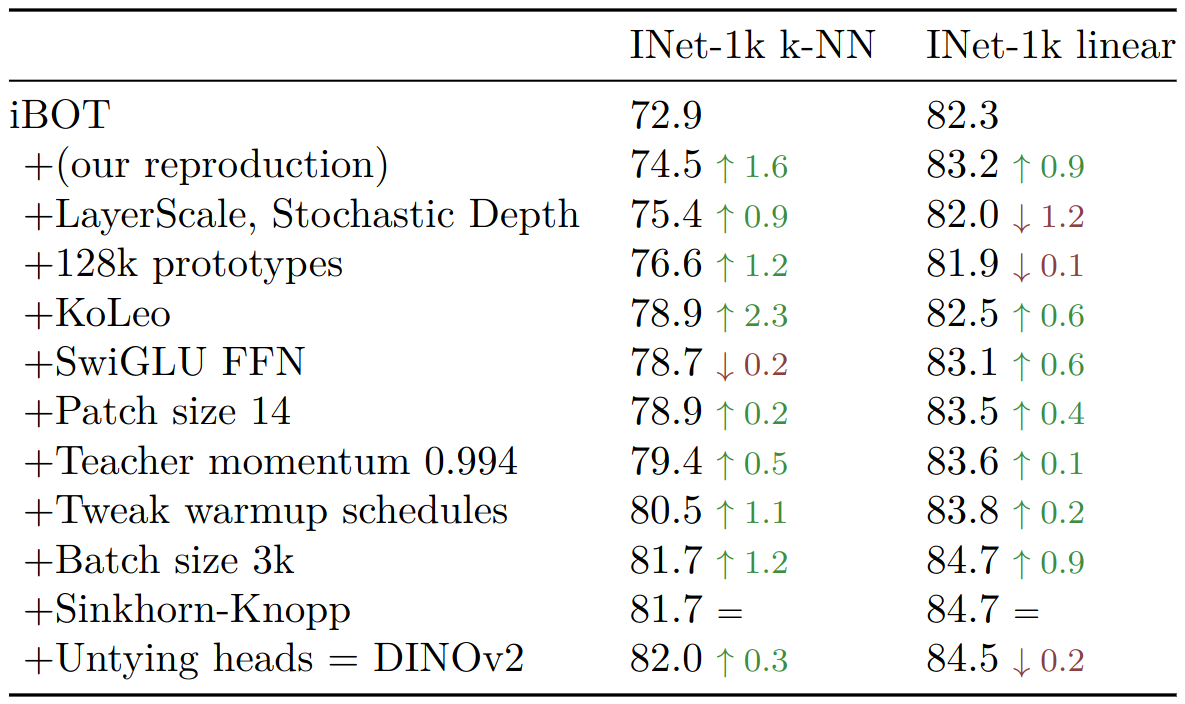
\includegraphics[height=70mm]{Immagini/ssl/res_dinov2.png}
    \caption{Un confronto fra iBOT e DINOv2. Si mostrano tutte le novità introdotte in quest'ultimo e il guadagno di prestazioni che comportano.}
    \label{tab:res_dinov2}
\end{table}

Le principali novità introdotte rispetto ad iBOT sono una serie di altre ottimizzazioni che migliorano le prestazioni del modello. Non si scenderà nei dettagli, di seguito solo un elenco di alcuni di essi e il loro apporto:
\begin{itemize}
    \item \textbf{Projection heads}: Gli autori osservano che, su scala più ampia, mantenere gli stessi pesi per le teste risulta penalizzante a livello di performance di classificazione, a differenza di iBOT, in cui migliorava i risultati. Per questo motivo, ogni testa ha dei pesi separati su cui verrà fatto l'addestramento.
    \item \textbf{Sinkhorn Knopp}: una forma migliorata di centering, per evitare il collasso.
    \item \textbf{Koleo Regularization}: un termine aggiunto alla loss che incoraggia una più uniforme distribuzione delle rappresentazioni su tutto lo spazio delle features.
    \item \textbf{Image Resolution}: durante il training, la dimensione delle immagini in input viene aumentata da 224x224 a 512x512 per migliorare per le performance in \textit{downstream tasks} a livello di pixel, come segmentazione e object detection. Permette di individuare oggetti che a basse risoluzioni risulterebbero troppo piccoli. 
\end{itemize}


